%!TEX root = ../report.tex

\chapter{Appendix: images}

\begin{figure}[ht]
\centering
\subfigure[The path of the robot according to the groundtruth, inertia sensor and SLAM]{
	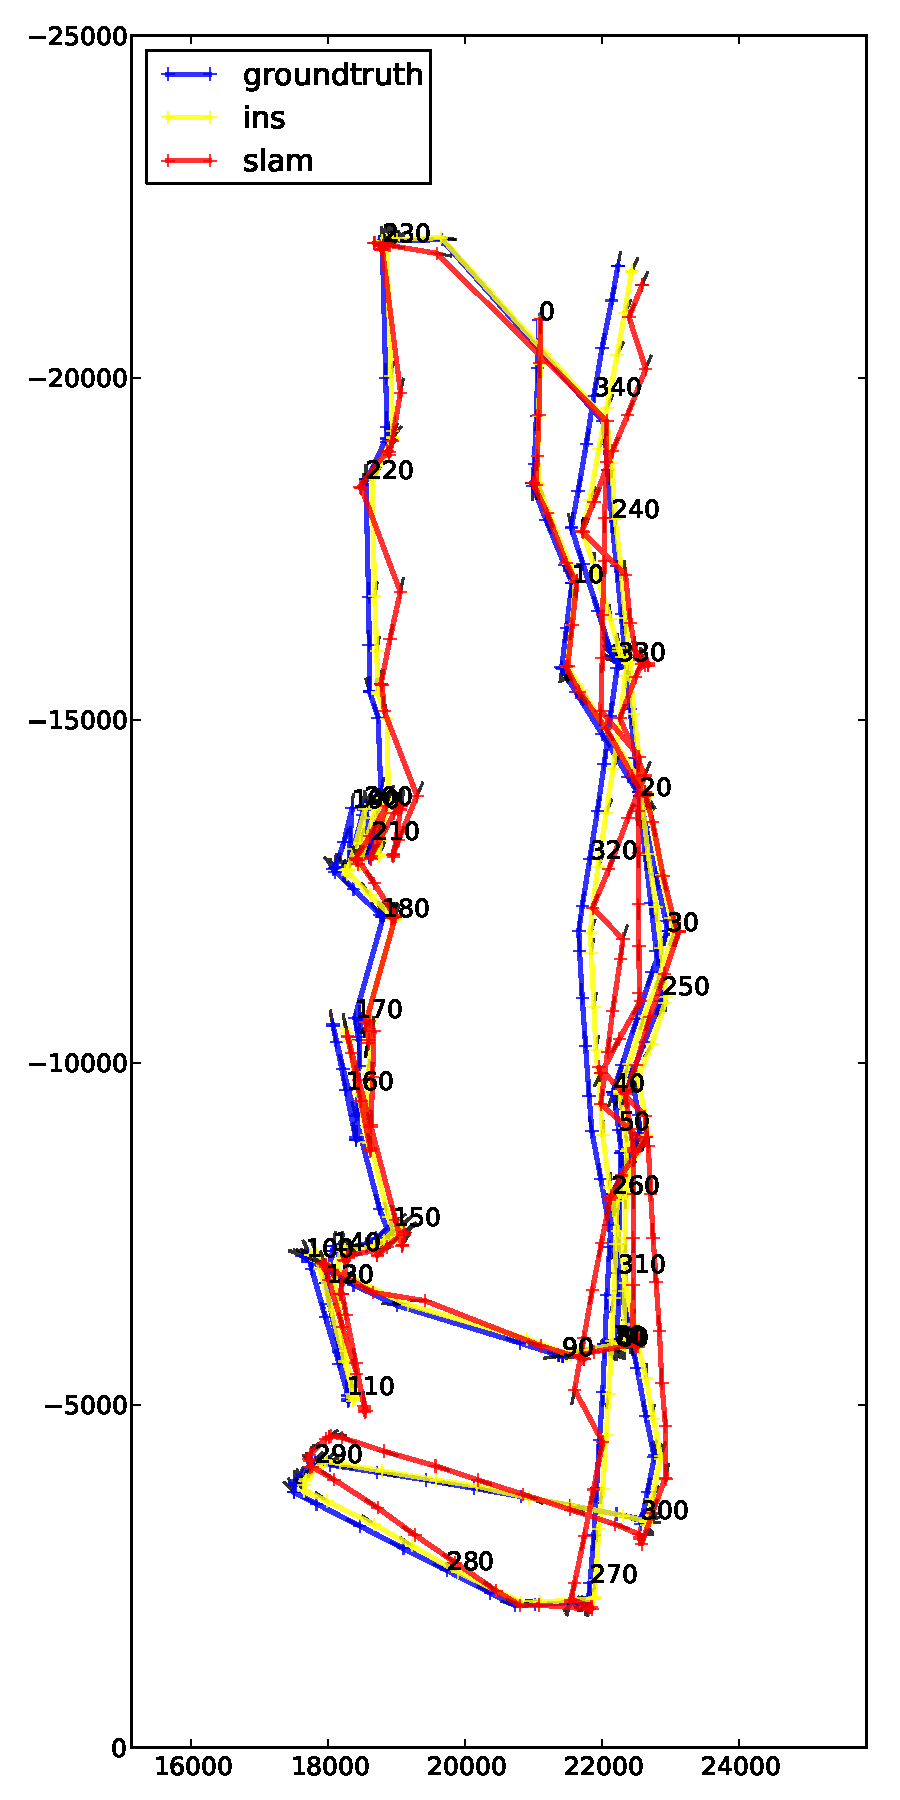
\includegraphics[width=0.45\textwidth]{images/experiment/map1/trace.pdf}
	\label{fig:apx:map1-paths}
}
\subfigure[The path of the robot according to SLAM, with associated uncertainty ellipsis. The error is plotted with yellow circles if there was infinite error (no matches at all).]{
	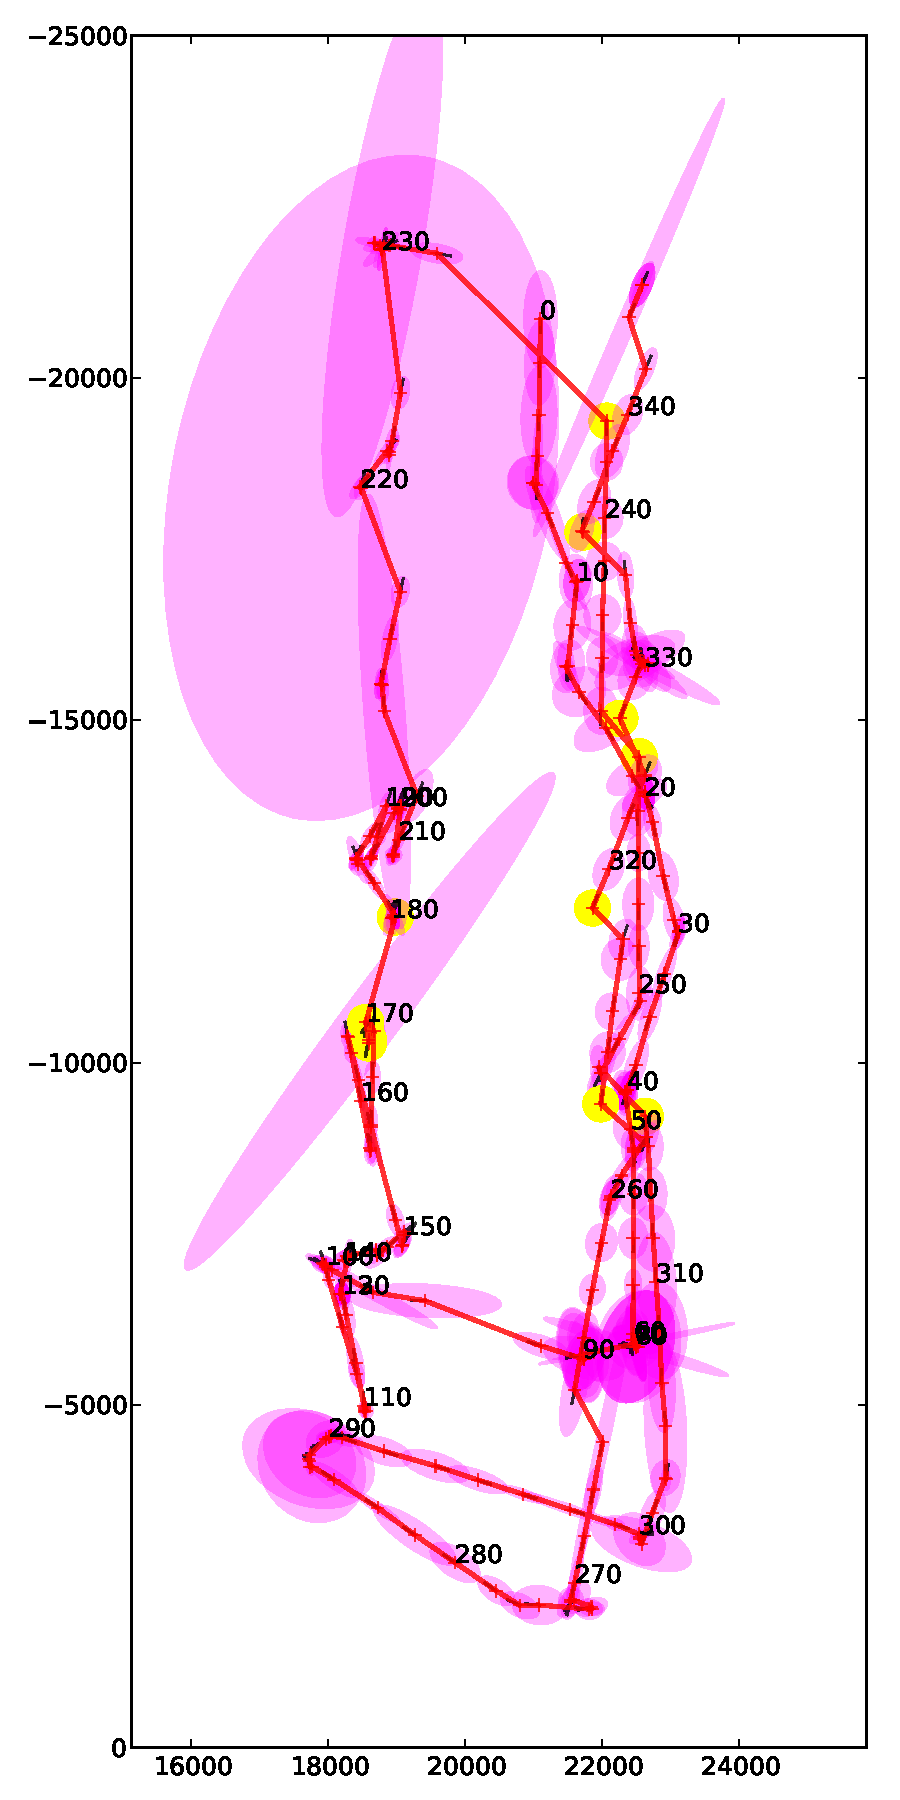
\includegraphics[width=0.45\textwidth]{images/experiment/map1/slam_covariance.pdf}
	\label{fig:apx:map1-trace}
}
\caption{Map 1 paths}
\label{fig:apx:map1}
\end{figure}

\begin{figure}[ht]
\centering
\subfigure[Piece 1: $0 \le t \le 65$]{
	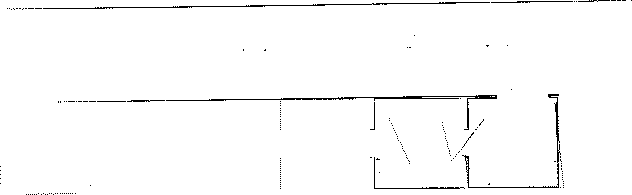
\includegraphics[resolution=144]{images/experiment/map1/maps/part-0-65-1.png}
}
\\
\subfigure[Piece 2: $69 \le t \le 95$]{
	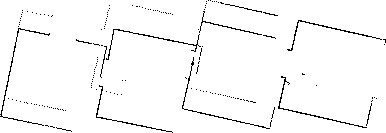
\includegraphics[resolution=144]{images/experiment/map1/maps/part-69-95-1.png}
}
%TODO: Add all other pieces
\caption{Map 1 parts}
\label{fig:apx:map1-pieces}
\end{figure}

part-0-65-1.png
part-69-95-1.png
part-97-102-1.png
part-104-112-1.png
part-114-158-1.png
part-160-163-1.png
part-165-167-1.png
part-169-174-1.png
part-176-182-1.png


% \subfigure[SLAM result]{
% 	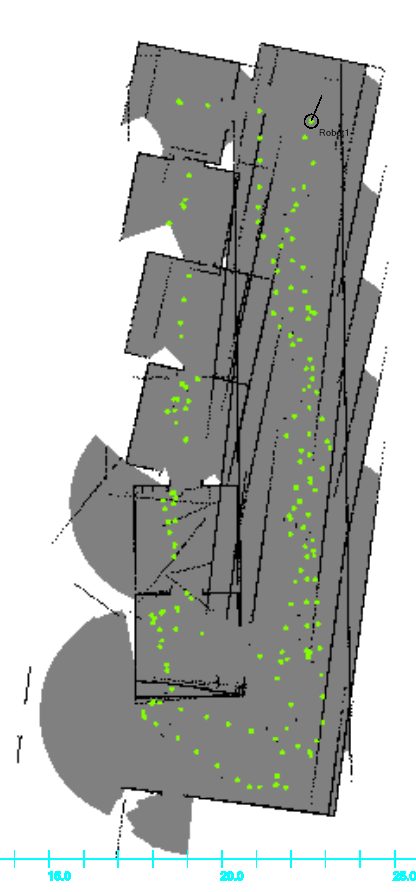
\includegraphics[width=0.45\textwidth]{images/experiment/map1/slam.png}
% 	\label{fig:apx:map1-trace}
% }